%\documentclass[12pt,fleqn, leqno, acm]{article}
\documentclass[12pt]{article}

%% Estilos e Plug-Ins
%\usepackage{a4wide}
\usepackage{a4}
\ifx\pdfoutput\undefined
   \usepackage[dvips]{graphicx}
\else
   \usepackage[pdftex]{graphicx}
\fi
\usepackage{times}
\usepackage[latin1]{inputenc}
\usepackage[brazil]{babel}
\usepackage{fancyheadings}
\usepackage{lastpage} 
\usepackage[T1]{fontenc}

\pagestyle{fancy}

\textheight=8.2in
%\headwidth=1.2\textwidth
\lhead{\setlength{\unitlength}{1mm} 
\begin{picture}(0,0) 
\put(0,0){
\includegraphics[width=0.8in]{figs/fundacao.pdf}} 
\end{picture}} 
\chead{\setlength{\unitlength}{1mm} 
\begin{picture}(0,0) 
\put(53,0){
\includegraphics[width=0.8in]{figs/tecgraf.pdf}} 
\end{picture}} 
\rhead{}

\lfoot{\scriptsize %
Tecgraf/PUC-Rio \hfill -
\hfill Rua Marqu�s de S�o Vicente, 225 - Pr�dio Velloso \hfill -
\hfill CEP 22453-900 \hfill - \hfill Rio de Janeiro -- Brasil\\
Tel. +55 21 512-5984 - Fax. +55 21 259-2232 \hfill -
\hfill E-mail: openbus@tecgraf.puc-rio.br \hfill -
\hfill URL: http://www.tecgraf.puc-rio.br\\
\vspace{0.5cm} 
\today \hfill P�gina \thepage \hspace{0.1cm} de \pageref{LastPage}} 
%27/6/2006	P�gina 1 de 33
\cfoot{}
\rfoot{}

\addtolength{\parskip}{\baselineskip}

\hyphenation{
}

\def \openbus {OpenBus}

% ===================
% In�cio do documento
% ===================
\begin{document}

\title{OpenBus -- Uma Arquitetura para Integra��o de Aplica��es}
\author{}
\date{}
\maketitle
\thispagestyle{empty}

\section{Introdu��o}
\label{introducao}

Os profissionais da �rea de Explora��o e Produ��o da Petrobras utilizam
 diversas aplica��es computacionais no desempenho de suas atividades t�cnicas.
Por exemplo, as tarefas relacionadas � aquisi��o, processamento e interpreta��o
 de dados s�smicos exigem a participa��o de diferentes profissionais, e cada
 profissional pode necessitar de v�rias aplica��es.
O fato de uma �nica aplica��o n�o dar suporte a todas as fases do trabalho e,
 �s vezes, nem mesmo a uma fase inteira, � fruto da elevada complexidade
 t�cnica inerente � manipula��o desses dados.
Essa complexidade se reflete diretamente nas aplica��es, for�ando um alto grau
 de especializa��o, e praticamente torna imposs�vel a constru��o de uma
 aplica��o que permeie todas as fases de trabalho sobre um dado.

Uma decorr�ncia direta dessa pluralidade de aplica��es utilizadas para a
 manipula��o de um dado � a necessidade de integra��o.
Afinal, para que o trabalho seja realizado, � preciso que os dados sejam
 migrados de uma aplica��o para outra, at� que o resultado final seja
 alcan�ado.
Em resumo, a capacidade de integra��o entre aplica��es � um suporte essencial
 para o trabalho dos profissionais da �rea de E\&P.

Ao longo de um ciclo de trabalho, um profissional carrega um dado em uma
 aplica��o e, atrav�s das funcionalidades providas por esta aplica��o, manipula
 o dado como necess�rio.
Em uma situa��o t�pica, o profissional manipula o dado at� o limite oferecido
 pela aplica��o e, ent�o, transporta o dado para outra aplica��o de forma a
 continuar seu trabalho.
Entretanto, na pr�tica, essa troca de dados entre duas aplica��es n�o
 necessariamente � feita de forma simples ou at� mesmo satisfat�ria.

Diferentes aplica��es da �rea de E\&P possuem formas pr�prias de representar e
 armazenar os dados.
Al�m disso, a quantidade e a variedade de atributos e meta-informa��es
 relacionadas a um mesmo tipo de dado tamb�m podem ser diferentes.
A falta de padroniza��o gera dificuldades na troca de dados entre as aplica��es
 que, muitas vezes, acaba sendo feita manualmente pelo pr�prio usu�rio.
A integra��o manual consiste na exporta��o dos dados em algum formato
 padronizado de arquivo na aplica��o de origem, a carga desse arquivo na
 aplica��o destino e os ajustes necess�rios para que eventuais informa��es
 adicionais, n�o representadas no arquivo gerado, sejam criadas corretamente no
 destino.
Essa forma de integra��o � fraca, pois obriga o usu�rio a assumir o papel de
 integrador e abre a possibilidade de perda das informa��es que porventura n�o
 sejam representadas no formato de arquivo utilizado.
Em uma situa��o extrema, as aplica��es podem n�o compartilhar um formato comum
 de arquivo, o que pode inviabilizar a troca de dados entre elas.

Quando as aplica��es s�o desenvolvidas internamente pela Petrobras, ou possuem
 c�digo aberto, ou, ainda, disp�em de interfaces para programa��o de extens�es,
 a integra��o por ser feita de forma program�tica direta.
Essa integra��o {\em ad hoc} entre duas aplica��es facilita substancialmente o
 trabalho do usu�rio que, ao inv�s de trocar arquivos e configura��es entre as
 aplica��es, apenas comanda a transfer�ncia dos dados.
Al�m disso, a integra��o program�tica pode considerar, al�m dos dados, os
 atributos e meta-informa��es que sejam comuns, ou convert�veis, entre as
 aplica��es, maximizando a qualidade do dado trocado e diminuindo as eventuais
 perdas de informa��es desse processo.
Essa forma de integra��o tamb�m est� presente, eventualmente, entre aplica��es
 de um mesmo fabricante, como � o caso das aplica��es de geologia e geof�sica
 da Landmark.

Dois exemplos de integra��o program�tica direta entre aplica��es pr�prias da
 Petrobras s�o a integra��o v3o2/WebSintesi e a WebSintesi/SIGEO.
A integra��o v3o2/WebSintesi � feita atrav�s de uma interface de acesso � �rea
 de projetos pr�pria do WebSintesi que � acessada pelo v3o2.
Dessa forma, o v3o2 tem acesso aos projetos do WebSintesi, podendo ler e
 escrever arquivos nos projetos.
A integra��o WebSintesi/SIGEO � feita de forma an�loga: uma interface de acesso
 espec�fica para aos projetos do SIGEO � acessada pelo WebSintesi que, atrav�s
 dela, consegue criar novos objetos nos projetos SIGEO.

A integra��o direta entre aplica��es �, sem d�vida, melhor do que a integra��o
 externa, feita pelo usu�rio atrav�s da troca de arquivos e ajustes manuais.
Entretanto, o esfor�o necess�rio na infra-estrutura para integrar as aplica��es
 � muito grande, pois precisamos codificar uma {\em ponte} espec�fica para
 ligar cada par de aplica��es.
Isso nos leva a um n�mero quadr�tico de codifica��es de pontes em rela��o ao
 n�mero de aplica��es.
A cada nova aplica��o a ser integrada, � preciso codificar uma ponte que
 integre esta nova aplica��o com cada uma das aplica��es j� existentes, o que
 significa (\(\frac{n(n-1)}{2}\)) codifica��es para {\em n} aplica��es.
Por exemplo, para integrar 10 aplica��es precisamos codificar 45 pontes.

Se a integra��o direta entre os pares de aplica��es demanda um esfor�o muito
 elevado, a ado��o de aplica��es de um mesmo fabricante, que possuem
 funcionalidades de integra��o intr�nsecas, � direta mas insuficiente.
Afinal, nenhum fabricante possui um conjunto de aplica��es que atenda a
 totalidade das funcionalidades exigidas pelos profissionais nos seus ciclos de
 trabalho.
Por outro lado, mesmo que um fabricante possu�sse tal conjunto de aplica��es,
 dificilmente sua ado��o seria desej�vel, dada a total depend�ncia que se
 estabeleceria deste fabricante.

Uma abordagem alternativa para as integra��es externa (via arquivos) e direta
 (via pontes entre os pares) � a ado��o de uma plataforma comum de integra��o
 entre aplica��es.
O princ�pio b�sico de uma plataforma de integra��o � definir um componente ou
 um {\em barramento} comum atrav�s do qual todas as aplica��es possam trocar
 dados.
Nesse modelo, cada aplica��o se conecta ao barramento, segundo um protocolo
 pr�prio deste barramento, e carrega ou exporta dados para outras aplica��es
 tamb�m conectadas ao barramento.

Como na integra��o direta, � necess�rio codificar uma ponte para conectar cada
 aplica��o ao barramento.
Tamb�m como na integra��o direta, o fato de se estabelecer uma interface e de
 se codificar uma ponte espec�fica, permite maximizar a qualidade do dado
 trocado entre as aplica��es, minimizando a eventual perda de informa��es
 decorrente da heterogeneidade dessas aplica��es.
Por outro lado, como o barramento define uma linguagem comum entre todas as
 aplica��es, a codifica��o de uma ponte entre uma aplica��o e o barramento � o
 suficiente para que esta aplica��o se integre a todas as demais aplica��es
 conectadas ao barramento.
Ou seja, diferente da abordagem de integra��o direta, onde o esfor�o de
 infra-estrutura � quadr�tico, a integra��o por meio de um barramento exige um
 esfor�o linear em fun��o do n�mero de aplica��es.
De fato, para integrar {\em n} aplica��es, � preciso codificar apenas {\em n}
 pontes.

Outra vantagem significativa da integra��o atrav�s de um barramento comum � a
 possibilidade de criarmos {\em liga��es ativas} entre as aplica��es.
Uma liga��o ativa � uma liga��o atrav�s da qual uma aplica��o pode perceber
 mudan�as nos dados de outra aplica��o.
Ou seja, por meio de uma liga��o ativa duas aplica��es podem trocar mensagens
 ao inv�s de apenas dados.
Atrav�s das liga��es ativas podemos criar integra��es onde as aplica��es
 trocam informa��es dinamicamente, � medida em que o usu�rio interage com cada
 uma.
Por exemplo, se uma aplica��o permite a visualiza��o de um dado proveniente de
 outra aplica��o, � poss�vel refletir na tela uma modifica��o que seja feita no
 dado original imediatamente ap�s essa modifica��o ter sido feita na aplica��o
 que hospeda esse dado.
Al�m disso, podemos explorar essa forma de comunica��o entre as aplica��es
 para, por exemplo, permitir o trabalho colaborativo entre usu�rios.

Na �rea de E\&P, existem solu��es de mercado que implementam arquiteturas de
 integra��o de aplica��es.
Entretanto, como veremos na se��o seguinte, essas solu��es s�o limitadas e n�o
 atendem a todos os requisitos de integra��o do E\&P da Petrobras.
Em fun��o dessas limita��es, e do fato desta abordagem de integra��o se mostrar
 como a mais adequada, n�s propomos, neste documento, a constru��o de uma
 arquitetura de integra��o baseada em um barramento, que chamamos de OpenBus.

Na se��o seguinte, al�m da apresenta��o e da an�lise das solu��es de mercado,
 n�s apresentamos as tecnologias que podem ser utilizadas na constru��o de uma
 arquitetura de integra��o e avaliamos cada uma em fun��o dos requisitos
 impostos pelas aplica��es de E\&P.
Na se��o \ref{arquitetura}, n�s descrevemos a arquitetura OpenBus,
 explicitando os requisitos contemplados e detalhando os servi�os que ser�o
 providos pela arquitetura.
Por fim, na se��o \ref{conclusoes}, conclu�mos este documento, sintetizando
 os benef�cios da arquitetura proposta.



\section{Estado da arte}
\subsection{Solu��es de mercado para a integra��o de dados e aplica��es de E\&P}
A solu��o para a integra��o de aplica��es de E\&P mais abrangente dispon�vel
no mercado � a plataforma OpenSpirit. O desenvolvimento dessa plataforma resultou de um cons�rcio
(a OpenSpirit Alliance),
que uniu esfor�os de diferentes companhias de petr�leo e fabricantes de
software para a defini��o de um {\em framework} de integra��o de aplica��es
que suportasse tanto o compartilhamento de dados mantidos em diferentes
reposit�rios, 
como tamb�m a colabora��o entre diferentes aplica��es.
Esse {\em framework} � comercializado hoje por uma companhia de software
independente (a OpenSpirit Foundation), que conta com um grupo de investidores
que inclui tanto companhias de petr�leo, como Chevron e Shell, como tamb�m
provedores de software e servi�os, como Schlumberger e Paradigm.

O {\em framework} OpenSpirit � composto por tr�s elementos principais:
o OpenSpirit Runtime, conectores de dados (Data Connectors)
e adaptadores de aplica��es (Application Adapters).
\begin{itemize}
\item OpenSpirit Runtime

O OpenSpirit Runtime prov� a infraestrutura de suporte para a integra��o de 
aplica��es e dados. Essa infraestrutura oferece uma s�rie de servi�os 
utilizados pelos
conectores de dados e adaptadores de aplica��es, como, 
por exemplo, a conex�o de uma aplica��o ao ambiente
de integra��o, a disponibiliza��o de informa��es sobre os reposit�rios de
dados acess�veis, e a difus�o de mensagens (eventos de colabora��o) entre
aplica��es. 

Para garantir a independ�ncia da plataforma de execu��o e da linguagem de
desenvolvimento das aplica��es 
--- um requisito essencial � ampla interoperabilidade pretendida 
pelo {\em framework} ---
a infraestrutura de suporte de integra��o implementada pelo OpenSpirit
� baseada no {\em middleware} CORBA, e em alguns dos servi�os padronizados
para sua arquitetura.

\item Conectores de Dados

Conectores de dados, ou {\em data servers}, s�o os elementos respons�veis por
implementar os servi�os de acesso aos diferentes reposit�rios, ou
{\em datastores}.
Esses conectores prov�em �s aplica��es uma vis�o uniforme e homog�nea dos
dados acessados, independente dos formatos internos adotados
por um cada tipo de reposit�rio.
Essa vis�o uniforme � baseada em um modelo de dados gen�rico 
(OpenSpirit Data Model),
oferecido pelos conectores de dados em sua interface de acesso;
� responsabilidade de cada tipo de conector realizar o mapeamento desse modelo
para um reposit�rio espec�fico.

� importante observar que o modelo de dados atualmente implementado 
pela OpenSpirit
� restrito ao dom�nio da Geologia e Geof�sica, o que impede
a integra��o de aplica��es de outros dom�nios, como Engenharia
e Qu�mica.
Al�m disso, apenas a pr�pria OpenSpirit desenvolve e comercializa 
conectores de dados; n�o existe um {\em toolkit} para o desenvolvimento
desses conectores.
Essa restri��o impede que reposit�rios de dados providos
por aplica��es e sistemas desenvolvidos pela Petrobras sejam incorporados
ao ambiente de integra��o, a menos que a pr�pria OpenSpirit seja
contratada para desenvolver os conectores necess�rios.

A OpenSpirit disponibiliza, atualmente, conectores 
para os seguintes reposit�rios: Open\-Works/Seisworks, GeoFrame/IESX/Charisma,
Finder,
GOCAD, Kingdom, Petra,
Managed SEGY (dados SEGY 2D e 3D armazenados em um sistema de arquivos),
Recall e ArcSDE.
Contudo, conectores espec�ficos podem n�o suportar
todos os tipos de dados de um reposit�rio;
o conector para o GOCAD, por exemplo, oferece por enquanto apenas o acesso a 
volumes s�smicos. 

\item Adaptadores de Aplica��es

Adaptadores de aplica��es (ou {\em application plug-ins}),
s�o os componentes respons�veis por integrar as diferentes aplica��es
ao ambiente OpenSpirit.
Esses componentes utilizam a
API oferecida pelo {\em toolkit} de desenvolvimento
para prover �s aplica��es o acesso aos servi�os de dados e de 
colabora��o disponibilizados pelo {\em framework}.
O {\em toolkit} de desenvolvimento � 
dispon�vel atualmente para diferentes linguagens (Java, C++, C\#, VB, Delphi)
e plataformas (Windows, Solaris, Linux, Irix).
Diversos fornecedores de software, como Schlumberger (Petrel),
Landmark (OpenWire), Earth Decision (Gocad) e Hampson-Russell (AVO),
prov�em adaptadores para suas aplica��es.
A pr�pria Petrobras � licenciada como desenvolvedor OpenSpirit,
e est� implementando para o WebSintesi/VGE
o acesso, via {\em framework} OpenSpirit, a reposit�rios de dados como 
Open\-Works/Seisworks e GeoFrame/IESX.

Como vimos anteriormente, os servi�os de acesso a dados s�o
oferecidos por conectores espec�ficos para cada reposit�rio.
Atrav�s de um mecanismo de {\em query} oferecido pela API, aplica��es podem 
criar, ler, atualizar
e remover dados com base no modelo de dados gen�rico oferecido por
esses conectores.
O mecanismo de {\em query}, contudo, n�o permite o acesso a {\em bulk data}, 
como volumes s�smicos e horizontes 3D. Para esse tipo de acesso, 
a API prov� a representa��o dos dados como objetos remotos.

A colabora��o entre aplica��es � baseada em 
um servi�o de difus�o de mensagens (notifica��es),
oferecido pelo OpenSpirit Runtime.
Esse servi�o permite que aplica��es 
que operam sobre um mesmo conjunto de dados
compartilhamem {\em eventos} 
de intera��o de usu�rio (sele��o e altera��o de dados, movimenta��o de cursor,
defini��o de �reas de interesse).
A API provida pelo {\em toolkit} oferece mecanismos para que as aplica��es
possam gerar e receber esses eventos, encapsulando o acesso ao
servi�o de notifica��es.

Um fator limitante para a colabora��o entre aplica��es atrav�s do 
{\em framework} � a restri��o do escopo dessa colabora��o
a uma sess�o OpenSpirit. Essa sess�o, determinada no momento de conex�o 
da aplica��o ao ambiente, estabelece tamb�m
o conjunto de dados, ou projetos ({\em ProjectSet}) acess�veis 
pela aplica��o durante a conex�o.
No ambiente de integra��o OpenSpirit, cada usu�rio ({\em userid}) � 
associado a uma configura��o particular, que inclui a defini��o das sess�es
�s quais as aplica��es iniciadas por esse usu�rio poder�o conectar-se.
Como sess�es n�o s�o compartilhadas entre usu�rios, n�o h� colabora��o entre
aplica��es iniciadas por usu�rios diferentes.

Al�m de eventos de colabora��o, o {\em framework} OpenSpirit permite 
que aplica��es recebam notifica��es de eventos de altera��o dos dados 
de um reposit�rio (cria��o, altera��o e remo��o),
enviada pelos conector correspondente.
Essa facilidade depende da capacidade do conector 
gerar esse tipo de evento; atualmente, apenas os conectores OpenWorks e Geoframe
possuem essa capacidade.

\end{itemize}
Uma outra solu��o dispon�vel no mercado para a integra��o de aplica��es e
reposit�rios de dados de E\&P � o PowerHub, comercializado pela Landmark.
Assim como o modelo de dados gen�rico implementado pelo {\em framework}
OpenSpirit, a plataforma PowerHub oferece um modelo de dados 
que abstrai formas de armazenamento propriet�rias,
permitindo �s aplica��es acessar de maneira uniforme dados providos 
por diferentes reposit�rios.

Diferentemente do {\em framework} OpenSpirit, � poss�vel desenvolver
conectores para a integra��o de reposit�rios de dados � plataforma PowerHub, o
que, em princ�pio, permitiria a integra��o de dados disponibilizados por
aplica��es e sistemas desenvolvidos pela Petrobras.
Contudo, a API para acesso aos reposit�rios
consiste apenas de uma interface de
{\em query} para acesso a bases de dados, baseada em Java JDBC;
essa API n�o oferece acesso a {\em bulk data}, como volumes s�smicos.
Para acessar esse tipo de dado, � necess�rio que as aplica��es implementem
seus pr�prios mecanismos, baseados em {\em toolkits} providos
pelos fornecedores das aplica��es que mant�m os reposit�rios.

Uma outra restri��o com respeito ao uso da plataforma PowerHub
como solu��o de integra��o de aplica��es e dados de E\&P � a imposi��o do 
uso da linguagem Java para a conex�o de aplica��es ao PowerHub.
Essa restri��o imp�e dificuldades relevantes para a integra��o de
diversas aplica��es desenvolvidadas pela Petrobras, como o SIGEO e o v3o2.

Finalmente, a plataforma PowerHub contempla apenas o acesso integrado a
diferentes reposit�rios de dados;
facilidades para a colabora��o entre aplica��es n�o s�o oferecidas
por essa plataforma.

(Falar do SeaBed? � uma proposta da Schlumberger para um modelo de 
dados maior, a OpenSpirit vai adotar...)

\subsection{Tecnologias para desenvolvimento de uma solu��o pr�pria}
Discutir solu��es de integra��o de aplica��es 
sem fazer refer�ncia ao conceito de 
arquitetura orientada a servi�os ({\em Service-Oriented Architecture}, ou SOA)
�, hoje, praticamente imposs�vel.
Apesar de n�o ser um conceito realmente novo, 
os benef�cios obtidos pela ado��o dos princ�pios de SOA para
a integra��o de aplica��es em ambientes heterog�neos
s�o cada vez mais reconhecidos no mercado,
tornando essa arquitetura um padr�o de refer�ncia
para a implementa��o de solu��es de integra��o.

Numa arquitetura SOA, aplica��es compartilham dados e funcionalidades
sob a forma de servi�os e interagem atuando como consumidores e/ou
provedores desses servi�os. 
A principal caracter�stica desse tipo de arquitetura � o baixo grau de 
acoplamento entre provedores e consumidores de servi�os.
Para atend�-la, os servi�os oferecidos devem ser descritos atrav�s de uma
linguagem independente de plataforma e linguagem de programa��o,
isolando o consumidor de um servi�o dos detalhes espec�ficos
de sua implementa��o. 
Esse tipo de descri��o ``neutra''\  permite, por exemplo, que consumidores e
provedores de servi�o sejam desenvolvidos em linguagens diferentes,
e executem sob diversas plataformas.
Al�m disso, a disponibiliza��o de um servi�o de registro, ou diret�rio,
permite que servidores publiquem suas ofertas de servi�o, 
e que consumidores desses servi�os possam pesquis�-las,
conhecer seus detalhes
e interagir com os servi�os,
sem conhecer, de antem�o, a identidade ou localiza��o de seus provedores.
Essa rela��o din�mica entre provedores e consumidores
de servi�o, ilustrada na Figura~\ref{figsoa},
confere ao ambiente um alto grau de reuso, extensibilidade, 
e de adapta��o a mudan�as.
\begin{figure}
\center
\includegraphics*{figs/figsoa.jpg}
\caption{Arquitetura orientada a servi�os}
\label{figsoa}
\end{figure}

A implementa��o de uma arquitetura SOA n�o pressup�e o uso de uma
tecnologia espec�fica;
qualquer tecnologia ou infraestrutura que d� suporte � descoberta 
din�mica de servi�os e � descri��o desses servi�os
com base em interfaces bem definidas e independentes de implementa��o
pode ser utilizada.
Contudo, a ado��o de padr�es abertos para a descri��o e publica��o
de servi�os e para a intera��o entre consumidores e provedores de
servi�os � fundamental para garantir a interoperabilidade em 
ambientes heterog�neos e a independ�ncia de fornecedores de tecnologias.
Nesse sentido, tanto servi�os WEB 
como a pr�pria arquitetura CORBA, tecnologias baseadas em padr�es abertos, 
independentes de fornecedor e de ampla aceita��o no mercado, 
s�o op��es a serem consideradas para a implementa��o de uma solu��o 
de integra��o multi-plataforma.
Uma outra op��o a ser considerada � Java Business Integration (JBI),
um padr�o para a implementa��o de uma arquitetura SOA
recentemente proposto pela Sun � comunidade Java.

\subsubsection{Servi�os WEB}
Servi�os WEB \cite{Newcomer2002} s�o, basicamente, envelopes
({\em wrappers})\  XML que encapsulam diversos tipos de sistemas de
software (objetos distribu�dos, sistemas de bancos de dados,
aplica��es WEB, aplica��es convencionais),
oferecendo formas  padronizadas para acesso aos dados e outras 
funcionalidades desses sistemas. 
O acesso a um servi�o WEB � realizado atrav�s do envio de mensagens
de requisi��o de servi�o representadas por documentos XML;
� responsabilidade da implementa��o da interface de um servi�o WEB
transformar essas mensagens XML para o formato apropriado
� invoca��o do sistema ou componente encapsulado e, quando for o caso,
criar a mensagem XML correspondente � resposta de uma requisi��o.

A tecnologia b�sica para a constru��o de servi�os WEB �, portanto, XML 
--- a linguagem � utilizada para descrever 
todo o tipo de dado, ou informa��o, envolvido na intera��o com esses servi�os.
Al�m de XML, uma infraestrutura de integra��o baseada em servi�os WEB envolve 
as seguintes tecnologias relacionadas:
\begin{itemize}
\item WSDL (Web Services Description Language)

� a linguagem utilizada para descrever a interface oferecida por um servi�o WEB.
Essa descri��o define os tipos de dados trocados entre consumidores e servi�os, 
as opera��es realizadas sobre esses dados e os mapeamentos ({\em bindings}) para os
protocolos utilizados no transporte das mensagens.

De forma geral, o mapeamento das funcionalidades de um determinado 
sistema para uma interface de servi�o WSDL n�o � uma tarefa trivial;
a descri��o WSDL de um servi�o � significativamente mais complexa que a interface 
``nativa'' desse servi�o.
Tipicamente, fornecedores de sistemas de banco de dados,
de infraestruturas de {\em middleware},
e de infraestruturas de integra��o baseadas em servi�os WEB prov�em ferramentas que
automatizam tanto a gera��o das descri��es de servi�o WSDL como tamb�m a
gera��o das implementa��es dessas interfaces (i.e, o mapeamento das intera��es
descritas pela interface WSDL para as invoca��es do componente encapsulado
pelo servi�o WEB).

\item SOAP (Simple Object Access Protocol)

� o protocolo utilizado para a troca de mensagens entre consumidores e 
servi�os WEB.
Mensagens SOAP s�o documentos XML transportadas geralmente em requisi��es e 
respostas HTTP; contudo, a defini��o do protocolo SOAP admite o uso de outros tipos de 
transporte.

\item UDDI (Universal Description, Discovery and Integration)

� o servi�o de registro utilizado para a publica��o dos servi�os WEB oferecidos
em um ambiente de integra��o. 
A especifica��o do {\em framework} UDDI define um modelo de dados em XML
para o armazenamento de informa��es sobre servi�os --- incluindo
a localiza��o de sua descri��o em WSDL ---
e APIs SOAP para a publica��o e consulta dessas informa��es.
\end{itemize}

A tecnologia de servi�os WEB d� suporte a dois padr�es b�sicos de 
intera��o:
baseada em chamada remota de procedimentos (RPC) e orientada a documento.
Numa intera��o baseada em RPC,
a mensagem XML enviada pelo consumidor de um servi�o 
representa uma chamada de m�todo
associada a par�metros de entrada e sa�da,
e produz uma resposta s�ncrona para esse consumidor.
Esse tipo de intera��o � geralmente observado quando 
sistemas de objetos distribu�dos
(como CORBA ou J2EE) ou outros tipos de sistemas com interfaces ``nativas''
baseadas em RPC
t�m suas interfaces mapeadas diretamente para interfaces WSDL.
Esse mapeamento, contudo, n�o exp�e toda a funcionalidade provida 
por um sistema de objetos distribu�dos \cite{Vinoski2002, Vogels2003}.
A tecnologia de servi�os WEB, por exemplo, n�o inclui
a no��o de refer�ncias a objetos,
essencial a padr�es de intera��o que requeiram a manuten��o
de estado entre requisi��es de servi�o.
Apesar de ser poss�vel expor objetos como servi�os
WEB, representando-os atrav�s de URIs
({\em Universal Resource Identifiers}),
requisitos mais r�gidos de escalabilidade e desempenho podem inviabilizar esse tipo de solu��o. 

No padr�o orientado a documento, a intera��o entre um consumidor e um
servi�o � ass�ncrona;
requisi��es de servi�o s�o mensagens XML auto-contidas e n�o envolvem
uma resposta imediata ao consumidor.
Esse tipo de intera��o � similar ao implementado, por exemplo, 
por sistemas de mensageria ({\em message-based systems}), 
e favorece um n�vel de integra��o de granularidade 
significativamente mais alto que o anterior.

A ado��o da tecnologia de servi�os WEB 
pode n�o ser adequada em alguns cen�rios de integra��o,
como o compartilhamento de dados de grande volume ---
dados s�smicos, por exemplo.
A representa��o desses dados em XML imp�e uma sobrecarga
relevante de processamento a consumidores e provedores
de dados,
al�m de um alto consumo da banda de comunica��o,
o que pode prejudicar o desempenho das aplica��es e do ambiente
de integra��o como um todo.
Al�m disso, 
dependendo do tamanho do dado acessado,
copi�-lo integralmente para clientes como
aplica��es de visualiza��o pode ser invi�vel.
Para atender esse tipo de cen�rio,
servi�os de acesso a reposit�rios usualmente disponibilizam
f�bricas de objetos que implementam diferentes m�todos para o acesso
estruturado aos dados.
Acessando esses objetos, o consumidor pode obter segmentos, 
ou por��es, do dado, � medida que forem necess�rios.
Conforme discutimos anteriormente, essa funcionalidade dificilmente � 
mapeada para interfaces de servi�os WEB.

De forma geral, a tecnologia de servi�os WEB � mais adequada 
a ambientes de alto n�vel de integra��o,
onde a intera��o entre consumidores e provedores de
servi�os � inerentemente
ass�ncrona,
interfaces de servi�o prov�em funcionalidades complexas
e desempenho de comunica��o n�o � um requisito essencial \cite{Vinoski20022}.
Essa propriedade n�o contempla
todas as caracter�sticas e requisitos para um ambiente de
integra��o de aplica��es e dados do E\&P da Petrobras. 

\subsubsection{Java Business Integration}
Java Business Integration (JBI) \cite{JBI2005} � uma proposta
para uma arquitetura de uma infraestrutura de integra��o 
baseada em Java e em princ�pios de SOA. 
Essa arquitetura, ilustrada na Figura~\ref{figjbi}, consiste, basicamente,
de um {\em container} ({\em JBI Environment}) que hospeda componentes 
dinamicamente conectados a um roteador de mensagens 
({\em Normalized Message Router}).
Esses componentes atuam no ambiente JBI como provedores ou
consumidores de servi�os, ou simultaneamente nos dois pap�is. 
Dois tipos distintos de componentes s�o definidos:
\begin{itemize}
\item {\em Service Engines}

S�o componentes que prov�em ou consomem servi�os internamente ao
ambiente JBI. Esse tipo de componente � respons�vel pela 
integra��o de aplica��es e sistemas implementados 
em Java
e de outros recursos acess�veis atrav�s de APIs dessa
linguagem, como, por exemplo, sistemas de banco de dados.
\item{\em Binding Components}

S�o componentes respons�veis pela integra��o 
de provedores e consumidores de servi�os externos ao
ambiente JBI ---
aplica��es ou sistemas implementados em 
outras linguagens, 
ou sobre outras plataformas.
Um {\em Binding Component} atua, basicamente,
como um representante do componente externo,
traduzindo os protocolos e formatos utilizados
na interface com esse componente para o padr�o adotado
no ambiente JBI.

\end{itemize}

\begin{figure}
\center
\includegraphics*{figs/figjbi.jpg}
\caption{Arquitetura JBI}
\label{figjbi}
\end{figure}

Assim como em uma infraestrutura baseada em servi�os WEB.
os componentes de um ambiente JBI interagem atrav�s de
um mecanismo de troca de mensagens baseado em XML,
e descrevem seus servi�os atrav�s de interfaces WSDL.
A interface de um servi�o compreende um conjunto de fun��es
--- opera��es WSDL --- que, dependendo do modelo de intera��o
especificado ({\em One-Way} ou {\em Request-Response}),
podem ou n�o produzir respostas s�ncronas ao consumidor do servi�o.

A intera��o entre componentes JBI
� mediada por um roteador de mensagens
--- {\em Normalized Message Router} (NMR).
� esse roteador quem recebe as mensagens geradas por um consumidor
ou provedor de servi�o e as direciona ao componente apropriado
ao seu processamento. 
Al�m de intermediar a troca de mensagens,
o NMR cumpre tamb�m o papel de servi�o de registro;
� atrav�s dele que provedores de servi�o
--- {\em Service Engines} e {\em Binding Components} ---
publicam suas interfaces WSDL e que consumidores 
obt�m as informa��es necess�rias para localizar
e interagir com esses servi�os.

Al�m da infraestrutura de suporte � intera��o entre componentes,
o padr�o JBI define tamb�m
mecanismos para a administra��o do ambiente de integra��o,
baseados em JMX ({\em Java Management Extensions}).
Esses mecanismos prov�em suporte para a instala��o de componentes,
para o controle de seu ciclo de vida e
para o gerenciamento do ambiente como um todo.

A arquitetura JBI � fortemente baseada na tecnologia de servi�os WEB
e, como essa tecnologia, privilegia ambientes de um alto n�vel de integra��o,
mostrando-se inadequada para os mesmos cen�rios que discutimos
anteriormente: o compartilhamento de dados bin�rios
e de grande volume e intera��es que requeiram suporte 
� manuten��o de estado entre requisi��es de servi�o.

Uma outra quest�o relevante � o foco da arquitetura JBI
na integra��o de aplica��es e sistemas baseados em Java.
Atualmente, grande parte das aplica��es e sistemas
utilizados na �rea de E\&P da Petrobras ---
tanto aplica��es pr�prias como aplica��es
de mercado --- � implementada em outras
linguagens.
A integra��o dessas aplica��es a um ambiente JBI
requer a implementa��o de 
{\em Binding Components}, de mecanismos de acesso
para a comunica��o entre as aplica��es e esses componentes
e de mecanismos de tradu��o entre as interfaces internas
e externas ao ambiente JBI.

\subsubsection{Arquitetura CORBA}
\label{CORBA}
A arquitetura CORBA \cite{Bolton2002} foi criada, em meados da d�cada de 90,
em resposta a uma demanda crescente por uma infraestrutura para o
desenvolvimento de aplica��es distribu�das em ambientes heterog�neos.
At� o in�cio dos anos 2000, o desenvolvimento e evolu��o de CORBA
recebeu um enorme suporte da ind�stria, refletido nas centenas de membros
da OMG --- a organiza��o respons�vel pela especifica��o dos padr�es
adotados para essa arquitetura.
Diversas implementa��es comerciais de CORBA foram oferecidas e utilizadas para
o desenvolvimento de aplica��es e sistemas distribu�dos em diferentes 
dom�nios, como com�rcio eletr�nico, telecomunica��es, aplica��es banc�rias
e cient�ficas e sistemas de tempo real.
Implementa��es abertas, bastante completas e de qualidade --- como MICO
e JacORB --- tamb�m contribu�ram fortemente para o sucesso dessa arquitetura. 

Nos �ltimos anos observa-se, por�m, uma redu��o no 
uso de CORBA e o redirecionamento de parte do mercado para outras tecnologias.
Esse redirecionamento deve-se, em grande parte, a dois fatores
principais.
O primeiro deles � o uso crescente da linguagem Java e de suas
plataformas pr�prias para a constru��o de sistemas distribu�dos,
como J2EE.
Entretanto,
plataformas centradas em uma linguagem n�o s�o
adequadas a ambientes predominantemente heterog�neos;
a integra��o de aplica��es desenvolvidas
em outras linguagens requer a implementa��o de 
adaptadores, o que implica um maior esfor�o
de desenvolvimento e, usualmente, preju�zos de desempenho.

O segundo fator foi a introdu��o da tecnologia de servi�os WEB
e sua identifica��o com os benef�cios de SOA.
Apesar de sua adequa��o a alguns cen�rios de integra��o,
essa tecnologia, como discutimos anteriormente,
n�o oferece as mesmas caracter�sticas e funcionalidades de 
um sistema de objetos distribu�dos, muitas delas necess�rias
� implementa��o de uma infraestrutura de integra��o com
requisitos espec�ficos, como � o caso da integra��o de
aplica��es de E\&P.

A redu��o observada no uso de CORBA � natural se considerarmos que
esta tecnologia existe e vem sendo trabalhada h� mais de uma d�cada.
� um comportamento t�pico de grandes parcelas do mercado---os chamados
{\em early adopters} e {\em early majority adopters}---a ado��o de novas
tecnologias, sem que isso represente uma real necessidade, mas movidos
pelo sentimento de estarem ``atualizados'' tecnologicamente.
Em contra partida, outros segmentos do mercado, os {\em late adopters},
adotam esta tecnologia atualmente, principalmente por verem em CORBA
uma tecnologia madura, comprovadamente est�vel e eficiente.
Em resumo, CORBA ainda � uma op��o vi�vel e segura para a constru��o
de sistemas distribu�dos \cite{Vinoski2004}.

CORBA �, basicamente, uma tecnologia de objetos distribu�dos
cuja principal caracter�stica � a independ�ncia de plataforma e
linguagem de programa��o.
Essa independ�ncia � garantida atrav�s do uso de uma linguagem neutra (IDL)
para a descri��o das interfaces de servi�o oferecidas por um objeto
--- isto �, as opera��es disponibilizadas e os tipos de dados que representam
os par�metros de entrada e sa�da definidos para essas opera��es.
Interfaces de servi�o descritas em IDL s�o significativamente
mais claras e sucintas que interfaces WSDL, permitindo, por exemplo, uma
melhor compreens�o das intera��es entre consumidores
e provedores de um determinado servi�o.

O padr�o CORBA define o mapeamento de IDL para 
as principais linguagens de programa��o utilizadas atualmente,
como C, C++, Java e Python, dentre outras.
Implementa��es de CORBA tipicamente oferecem compiladores que
traduzem interfaces IDL para linguagens espec�ficas,
produzindo o c�digo que permite que clientes e provedores
de servi�o desenvolvidos nessas linguagens possam invocar e atender 
as opera��es definidas em IDL.
Como os mapeamentos de IDL s�o padronizados,
implementa��es de clientes e servidores independem do compilador
de um fornecedor espec�fico, e podem ser portadas sem qualquer
altera��o.

Para garantir a interoperabilidade entre diferentes implementa��es 
da arquitetura CORBA, o transporte de requisi��es de servi�o e 
de suas respostas utiliza um protocolo padronizado pela OMG (IIOP).
A especifica��o desse protocolo define o formato das mensagens
trocadas, a representa��o dos dados transportados nessas mensagens,
e o mapeamento da comunica��o sobre conex�es TCP/IP% 
\footnote{IIOP �, na verdade, a especializa��o de um protocolo gen�rico (GIOP),
que n�o especifica um protocolo de transporte espec�fico,
apenas um conjunto de requisitos, como o suporte a conex�es bi-direcionais.}.
O projeto desse protocolo levou em considera��o uma s�rie de requisitos,
dentre eles escalabilidade e desempenho.
Ao contr�rio de SOAP, por exemplo, que utiliza XML (uma representa��o 
textual), o protocolo IIOP utiliza uma representa��o mais adequada
ao transporte eficiente de diversos tipos de dados, inclusive dados
bin�rios.  
Essa caracter�stica, aliada � disponibilidade de implementa��es de CORBA
de grande desempenho,
explica o sucesso e a predomin�ncia dessa arquitetura 
em dom�nios como sistemas de tempo real e sistemas embutidos.

Al�m da infraestrutura para suporte � intera��o entre
clientes e provedores de servi�o, o padr�o CORBA define tamb�m
uma s�rie de servi�os b�sicos, dentre eles um servi�o de nomes
e um servi�o de {\em trading}

A fun��o b�sica do servi�o de nomes � permitir que clientes de um 
servi�o obtenham dinamicamente a localiza��o --- isto �, a refer�ncia 
--- dos objetos que constituem os pontos de acesso a esse servi�o.
Para prover essa funcionalidade, o servi�o de nomes mant�m um
reposit�rio que armazena associa��es ({\em bindings}) entre nomes
e refer�ncias de objetos.
Provedores de servi�os fornecem ao servi�o de nomes essas associa��es;
clientes de servi�os utilizam o servi�o de nomes para
obter a localiza��o do objeto associado a um determinado nome.

O servi�o de {\em trading} oferece uma funcionalidade mais rica
para a descoberta de provedores de servi�os, permitindo
a associa��o de caracter�sticas, ou propriedades,
�s ofertas de um tipo de servi�o (uma interface).
Ao exportar uma oferta de servi�o, um provedor especifica,
al�m de sua interface e localiza��o, valores para essas propriedades.
Atrav�s de consultas ao servi�o de {\em trading}, consumidores
de um servi�o podem obter a localiza��o de um ou mais provedores que 
satisfa�am determinados crit�rios --- restri��es ou condi��es quanto
aos valores das propriedades.

A especifica��o de interfaces de servi�o em um linguagem neutra (IDL)
e a possibilidade de descoberta din�mica de provedores de servi�o,
seja atrav�s do servi�o de nomes ou do servi�o de {\em trading},
prov�em o suporte necess�rio para a implementa��o de uma arquitetura
SOA baseada em CORBA.
CORBA
prov� tamb�m todas as facilidades de uma tecnologia de 
objetos distribu�dos: o suporte a refer�ncias a objetos,
� instancia��o de objetos a partir de f�bricas
e � manuten��o de estado ao longo de intera��es entre consumidores
e provedores de servi�o.
Essas caracter�sticas, aliadas a um transporte mais eficiente 
de dados bin�rios e de grande volume,
permitem que uma infraestrutura baseada em CORBA
atenda aos requisitos necess�rios
� integra��o de aplica��es de E\&P.

O padr�o CORBA define tamb�m
dois servi�os que prov�em suporte � troca ass�ncrona de 
mensagens gen�ricas: o servi�o de eventos e o servi�o de 
notifica��es.
Esses servi�os 
disponibilizam canais de comunica��o que 
atuam como roteadores, intermediando a intera��o
entre geradores e consumidores de mensagens.
Geradores e receptores de mensagens s�o fortemente desacoplados.
Um gerador envia suas mensagens a um canal de comunica��o, 
sem necessariamente conhecer a identidade ou localiza��o de
poss�veis consumidores.
Consumidores de mensagens, por sua vez, recebem mensagens 
de um canal sem necessariamente conhecer a identidade ou localiza��o 
de seus geradores.
O estabelecimento de um canal de comunica��o
n�o exige uma correspond�ncia de um para
um entre geradores e consumidores de mensagens;
a conex�o de m�ltiplos geradores e de m�ltiplos consumidores a
um mesmo canal de comunica��o � permitida.

O servi�o de notifica��es estende a funcionalidade b�sica do
servi�o de eventos --- a troca ass�ncrona de mensagens gen�ricas ---
oferecendo algumas facilidades adicionais, como, por exemplo,
a defini��o de eventos estruturados,
a possibilidade de um consumidor especificar filtros para
restringir o tipo de eventos que deseja receber,
e a configura��o de diversas  propriedades de qualidade
de servi�o --- como garantia de entrega, prioridade e 
tempo de vida de mensagens.   

O suporte � troca de mensagens ass�ncronas entre aplica��es
� uma funcionalidade importante para ambientes de integra��o.
Al�m de permitir, quando adequado, um maior desacoplamento
entre provedores e consumidores de servi�o,
essa funcionalidade � essencial a aplica��es que desejam
implementar facilidades de colabora��o.


\section{Proposta}
\label{proposta}

Conforme discutimos na se��o anterior, duas ferramentas de mercado objetivam
 a integra��o de aplica��es da �rea de E\&P, OpenSpirit e PowerHub.
Entretanto, nenhuma das duas pode ser adotada como ferramenta de integra��o das
 aplica��es de E\&P da Petrobras.
No caso do OpenSpirit, a raz�o t�cnica que inviabiliza sua ado��o � o fato
 desta ferramenta n�o permitir a cria��o de um provedor de dados, o que
 significa que n�o � poss�vel disponibilizar em seu barramento os dados das
 v�rias bases de dados e aplica��es pr�prias da Petrobras.
J� no caso do PowerHub, h� duas quest�es t�cnicas impeditivas: o fato desta
 ferramenta n�o prover suporte para a troca de alguns tipos de dados---que � o
 objetivo principal da integra��o desejada---e o fato de estar restrita �
 linguagem Java.

Pelo lado n�o t�cnico, adotar uma ferramenta de mercado como infra-estrutura de
 integra��o das bases de dados e das aplica��es de E\&P tamb�m pode n�o ser
 desej�vel.
Usar uma ferramenta de mercado significa criar uma depend�ncia significativa,
 no sentido de que todas as aplica��es que forem integradas passam a conter
 c�digo espec�fico dessa ferramenta.
Mais do que isso, todo o fluxo de trabalho dos profissionais passa a depender
 do uso dessa infra-estrutura.
Assim, abandonar essa ferramenta no futuro significaria despender um grande
 esfor�o, tanto na atualiza��o das aplica��es quanto em fun��o do
 comprometimento dos fluxos de trabalho.
Motivos poss�veis para uma eventual interrup��o do uso s�o o aumento dos custos
 das licen�as, a descontinuidade da ferramenta por parte do fabricante ou mesmo
 a inadequa��o, tendo em vista que o fabricante s� incorpora funcionalidades
 que julga conveniente ao produto.
Como exemplos de inadequa��o, podemos citar o fato do OpenSpirit n�o permitir
 a colabora��o entre aplica��es de diferentes usu�rios e a possibilidade de n�o
 contemplar um determinado tipo de dado necess�rio ao ambiente da Petrobras.

Em fun��o dessas quest�es, n�s propomos a constru��o de uma nova arquitetura de
 integra��o de aplica��es, baseada em um barramento de servi�os, pr�pria da
 Petrobras, que chamamos de \openbus.
Com uma arquitetura pr�pria, todos os requisitos relevantes do ambiente da
 Petrobras poder�o ser contemplados.
Al�m disso, a arquitetura poder� ser mantida e estendida, de modo a contemplar
 novos requisitos que vejam a surgir, se adequando �s necessidades futuras.

O desenvolvimento de uma arquitetura de integra��o e sua ado��o nas aplica��es
 representa uma tarefa de esfor�o consider�vel.
A infra-estrutura, envolvendo o servidor e os servi�os b�sicos a serem
 providos, � complexa e a constru��o das pontes que ligam cada aplica��o ao
 barramento envolvem conhecimentos espec�ficos destas aplica��es.
Em fun��o do esfor�o n�o ser pequeno, � importante que o ponto de partida deste
 trabalho seja:
\begin{enumerate}
\item O levantamento dos requisitos a serem contemplados pela arquitetura.
\item A defini��o das tecnologias a serem empregadas na implementa��o.
\end{enumerate}

Na elabora��o desta proposta, definimos os seguintes requisitos para o
 \openbus:

\begin{description}
\item [Arquitetura aberta e extens�vel a diferentes dom�nios.] O E\&P abrange
 v�rias �reas de conhecimento al�m de geologia e geof�sica. Al�m disso,
 considerando a empresa inteira, h� in�meras �reas nas quais a exist�ncia de
 uma arquitetura de integra��o de aplica��es seria de grande valia. Assim, um
 dos requisitos do \openbus\/ � que ele seja flex�vel para atender diferentes
 dom�nios. Por exemplo, deve ser poss�vel montar um integrador de aplica��es
 de engenharia reaproveitando toda a infra-estrutura e os servi�os b�sicos que
 ser�o desenvolvidos inicialmente para aplicar em geologia e geof�sica.
\item [Dados estruturados e adequados ao dom�nio.] � importante que os dados
 sejam modelados de forma estruturada e de acordo com o dom�nio para permitir
 que as aplica��es naveguem por estes dados, encontrem e recuperem as
 informa��es desejadas. Esse requisito � fundamental para permitirmos que dados
 de grandes volumes possam ser utilizados. Por exemplo, um volume s�smico deve
 ser visto conforme sua estrutura l�gica, dividido em atributos, {\em inlines}
 e {\em crosslines}, ao inv�s de uma mera seq��ncia de bytes, como armazenado
 em um arquivo no formato {\em seg-y}.
\item [Compat�vel com m�ltiplas linguagens.] Para integrar de forma nativa e,
 em decorr�ncia, eficiente as aplica��es pr�prias da Petrobras, � necess�rio
 que o \openbus\/ seja independente de linguagem de programa��o, pois h� v�rias
 aplica��es escritas em C, C++, Java, .NET etc. Deve ser poss�vel conectar
 todas essas aplica��es ao barramento.
\item [Facilidade para cria��o de clientes.] A exemplo do que � feito pelo
 OpenSpirit, � interessante prover bibliotecas, nas principais linguagens de
 desenvolvimento, que facilitem a constru��o de pontes ligando aplica��es ao
 barramento. Esse requisito � importante para permitir que os pr�prios
 programadores das aplica��es possam conect�-las ao ambiente integrador.
\item [Facilidade para cria��o de servidores de dados.] � fundamental que
 possamos disponibilizar no barramento os dados de qualquer banco ou aplica��o
 pr�pria da Petrobras. Assim viabilizamos o maior grau de integra��o poss�vel
 entre as diferentes aplica��es.
\item [Troca de dados e mensagens entre as aplica��es.] A troca de dados entre
 as aplica��es � o objetivo principal da arquitetura de integra��o. Por�m, a
 troca de mensagens gen�ricas, de forma s�ncrona e ass�ncrona, permite aumentar
 significativamente as possibilidades de integra��o entre essas aplica��es.
\item [Efici�ncia da troca de grandes volumes de dados.] Os dados s�smicos s�o
 da ordem de grandeza de centenas de Gigabytes e precisam ser trocados entre as
 aplica��es dos dom�nios de geologia e geof�sica. A transfer�ncia desses
 dados n�o devem apenas ser permitida mas deve ser o mais eficiente poss�vel.
\item [Escalabilidade na troca de grandes volumes de mensagens.] A troca de
 mensagens, con\-for\-me apresentamos, flexibiliza as funcionalidades
 decorrentes da integra��o. Por exemplo, atrav�s da troca de mensagens, duas
 aplica��es podem sincronizar altera��es simult�neas sendo feitas em um mesmo
 dado que seja visualizado em ambas. Esse tipo de uso pode exigir grandes
 volumes de mensagens e a arquitetura deve dar suporte, sem degrada��o de
 desempenho do sistema.
\item [Suporte a mecanismos de autentica��o e autoriza��o.] Em praticamente
 qualquer �rea da Petrobras, a seguran�a da informa��o � essencial. O
 \openbus\/ deve, ent�o, dar suporte para que a autentica��o dos usu�rios e a
 autoriza��o de acesso a dados e servi�os sejam feitos conforme necess�rio.
\item [Suporte ao trabalho colaborativo.] A integra��o de aplica��es para a
 troca de dados, aliada � troca de mensagens que citamos acima formam uma base
 para o trabalho colaborativo entre usu�rios. A arquitetura pode, ent�o,
 oferecer os servi�os b�sicos, no n�vel de abstra��o adequado, para as
 aplica��es que desejem explorar a colabora��o.
\end{description}

Especificados os requisitos, passamos � defini��o das tecnologias a serem
 utilizadas na implementa��o do \openbus.
A constru��o de um barramento comum atrav�s do qual aplica��es possam se
 conectar para trocar dados e mensagens, como descrevemos, j� sugere uma
 abordagem baseada em servi�os, ou um SOA.
Uma arquitetura SOA atende � solu��o que propomos por garantir um alto grau
 de desacoplamento entre os membros do barramento, viabilizando a integra��o
 de aplica��es heterog�neas, e por n�o implicar em uma tecnologia espec�fica
 para sua implementa��o, nos permitindo adotar uma que atenda aos requisitos
 funcionais, ainda considerando desempenho e escalabilidade.
Al�m de atender aos requisitos t�cnicos espec�ficos, a ado��o de uma
 arquitetura orientada a servi�os tamb�m atende �s diretrizes estabelecidas
 pela TI-IDTA-AT em \cite{petrobras}.

Com base nos requisitos levantados, a tecnologia que julgamos mais adequada �
 implementa��o do \openbus\/ � CORBA.
Como apresentamos na se��o anterior, COR\-BA possui todos os requisitos para uma
 implementa��o de SOA.
Al�m disso, CORBA oferece suporte para descri��o clara e sucinta das interfaces
 dos servi�os, � constru��o de componentes em m�ltiplas linguagens, �
 mensageria, � implementa��o de mecanismos de autentica��o e ao acesso, via
 refer�ncias, a objetos remotos que podem preservar estado.
Por fim, CORBA possibilita um desempenho muito superior quando comparado com as
 tecnologias que adotam comunica��o baseada em XML.

Na pr�xima se��o, n�s apresentamos a arquitetura proposta para o \openbus,
 descrevendo suas macro-funcionalidades e os servi�os b�sicos que estar�o
 dispon�veis para as aplica��es.


\section{Arquitetura}
\label{arquitetura}

O \openbus\/ � baseado no {\em middleware} CORBA
e em alguns dos servi�os padronizados para sua arquitetura.
Seu barramento � formado por componentes que podem oferecer
servi�os ou podem apenas consultar servi�os de outros componentes.
A infraestrutura do \openbus\/ prov� alguns servi�os b�sicos que podem ser
oferecidos por um �nico componente ou podem estar
distribu�dos em diversos componentes em diferentes m�quinas.
A medida que as aplica��es se conectam ao barramento, o espa�o
de servi�os que o \openbus\/ oferece cresce. 
Desta forma, o \openbus\/ pode ser estendido com servi�os para acesso a
reposit�rios de dados (Base integrada, OpenSpirit),
acesso a dados de uma aplica��o (Websintesi, v3o2), etc.
(Figura~\ref{fig:architecture}.)

\begin{figure} [htb]
\centering
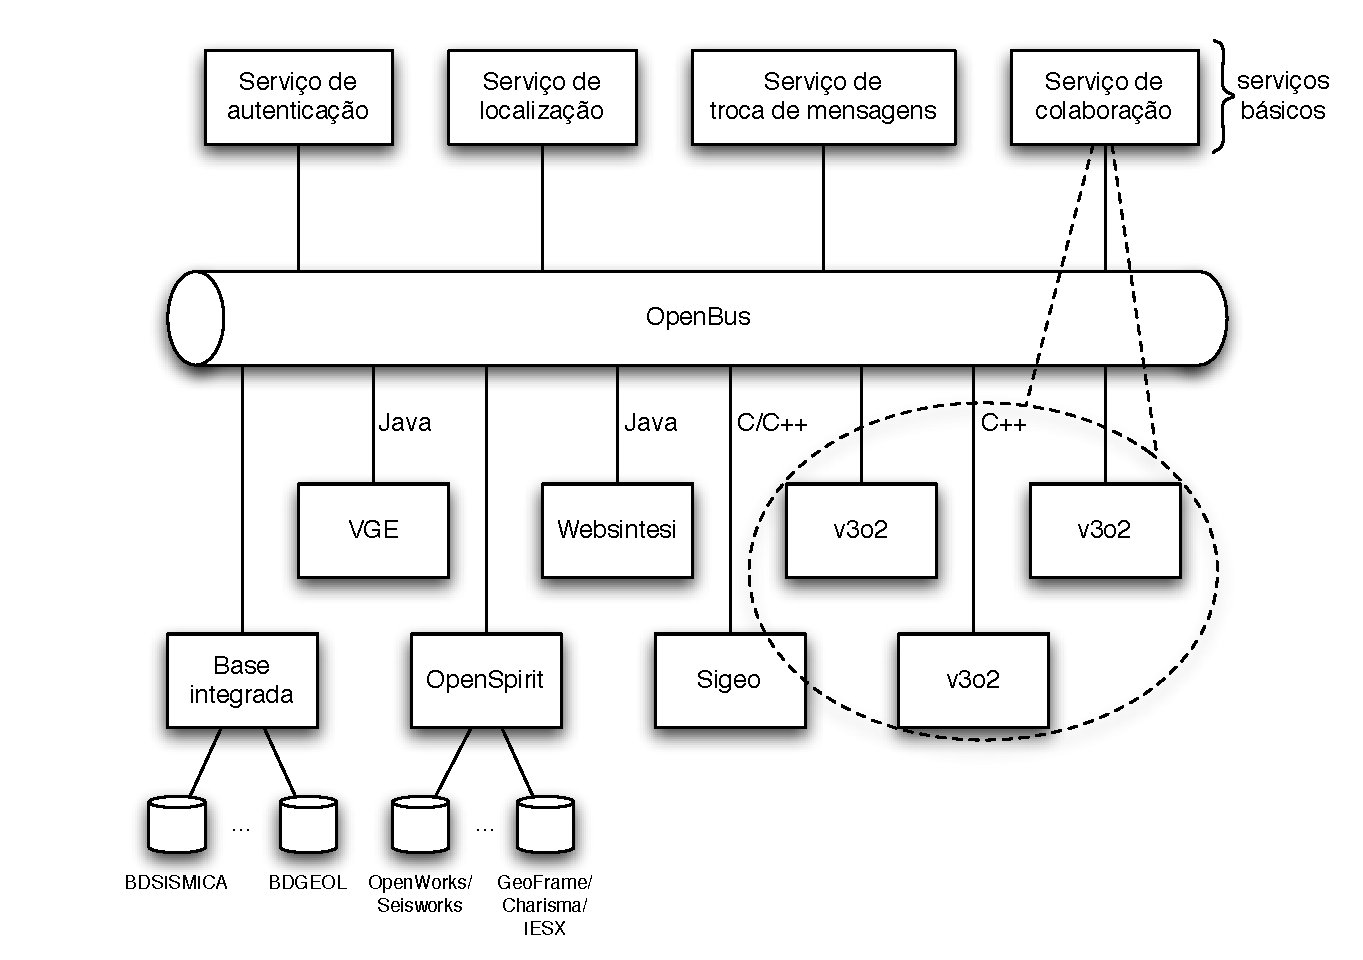
\includegraphics[width=14cm]{figs/arquitetura.pdf} %height=3in, 
\caption{Arquitetura do \openbus}
\label{fig:architecture}
\end{figure}

Qualquer aplica��o que queira fazer parte do barramento deve
implementar um componente para o \openbus. Atrav�s desse componente
� poss�vel acessar todos os servi�os existentes no barramento.
Para isso, o componente deve ser capaz de se conectar ao barramento e se
autenticar.
Atrav�s dos servi�os oferecidos pelo \openbus, o componente pode acessar
um servi�o previamente conhecido, ou pode consultar o servi�o de
localiza��o para descobrir qual componente oferece o servi�o que ele
deseja acessar.
Para oferecer um servi�o, uma aplica��o pode usar o mesmo componente ou
implementar outro. Tal componente deve ser capaz de publicar no
barramento a interface do servi�o que deseja oferecer.

%\subsection{Servi�os b�sicos}

Entre os servi�os b�sicos oferecidos pelo \openbus\/ podemos destacar os
servi�os de autentica��o, localiza��o, troca de mensagens e colabora��o.

\begin{itemize}
%%%%%%%%%%
\item Servi�o de autentica��o 
%%%%%%%%%%

Para fazer parte do barramento, um componente deve se autenticar a ele.
Existem tipicamente duas formas de autentica��o para um
componente. Uma onde o componente usa a credencial de um usu�rio e outra
onde o componente (ou aplica��o) possui uma credencial pr�pria.

Aplica��es como o VGE, onde o usu�rio fornece seu identificador e sua
senha, podem usar a pr�pria credencial do usu�rio para 
autenticar seus componentes no barramento.
J� as aplica��es que executam como um {\em daemon} podem utilizar uma
credencial pr�pria.

Como apenas um componente do barramento pode acessar servi�os de outro
componente e todos os componentes do barramento j� foram autenticados,
os componentes do barramento s�o considerados confi�veis.
Entretanto, cabe a cada servi�o verificar se um componente possui a
devida autoriza��o para acessar seus servi�os.

%%%%%%%%%%
\item Servi�o de localiza��o 
%%%%%%%%%%

O servi�o de localiza��o � baseado no servi�o de {\em trading} de 
CORBA. Este servi�o facilita a oferta e o descobrimento de inst�ncias de
servi�os de tipos espec�ficos.
Com este servi�o, componentes podem publicar suas caracter�sticas
e outros componentes podem encontrar os servi�os desejados
atrav�s das caracter�sticas publicadas.

Para publicar um servi�o, um componente prov� ao servi�o de localiza��o
uma descri��o de seu servi�o e a sua localiza��o.
Para encontrar um servi�o, um componente pergunta ao servi�o
de localiza��o se existe algum servi�o com determinadas caracter�sticas.
O servi�o de localiza��o procura entre as descri��es que possui e
responde com a localiza��o da interface do servi�o selecionado.
O componente que solicitou o servi�o pode ent�o acess�-lo.

%%%%%%%%%%
\item Servi�o de troca de mensagens
%%%%%%%%%%

O servi�o de troca de mensagens � baseado no servi�o de notifica��o de 
CORBA.
Atrav�s dele, as aplica��es podem comunicar-se livremente,
trocando mensagens diretas ou registrando interesse em receber 
mensagens quando algum even\-to ocorre na outra aplica��o.

Quando duas aplica��es est�o vendo o mesmo dado e uma delas o altera, 
atrav�s desse servi�o, ela pode enviar uma mensagem para a outra
aplica��o para que ela atualize a sua c�pia do dado.

%\begin{figure} [htb]
%\centering
%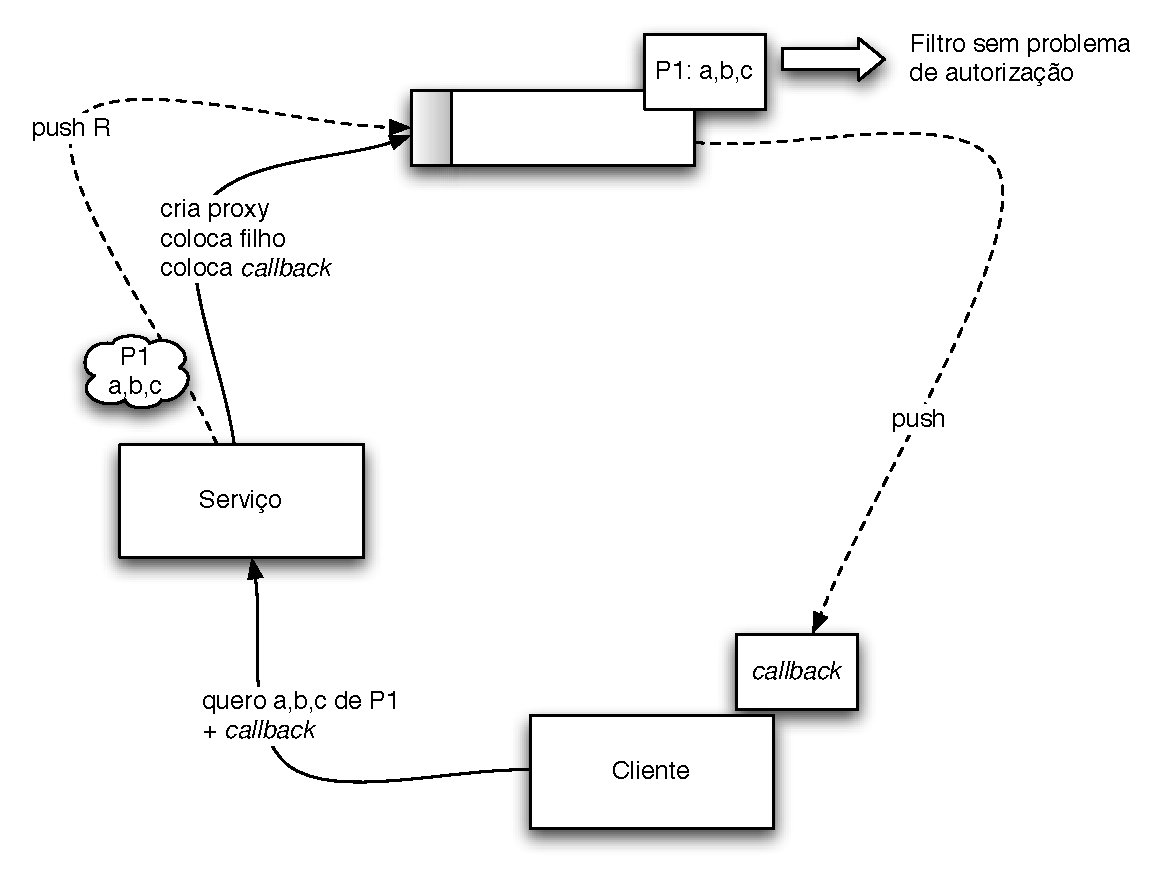
\includegraphics[width=8cm]{figs/eventos.pdf} %height=3in, 
%\caption{Troca de mensagens}
%\label{fig:datachange}
%\end{figure}

%%%%%%%%%%
\item Servi�o de colabora��o
%%%%%%%%%%

O servi�o de colabora��o usa o servi�o de troca de mensagens.
Atrav�s dele, um componente pode criar uma se��o de
colabora��o definir quem s�o os componentes participantes.
Inicialmente, cada componente � convidado pelo servi�o de colabora��o
a fazer parte desta se��o.

Cada se��o de colabora��o possui atributos espec�ficos e pode envolver
mais de um tipo de aplica��o de diferentes usu�rios.
Por exemplo, uma colabora��o entre diferentes inst�ncias 
do v3o2 pode ter atributos de c�mera, para que as diferentes inst�ncias
tenham a mesma vis�o do volume (Figura~\ref{fig:architecture}.)
Atrav�s de uma se��o, os componentes envolvidos podem compartilhar
diferentes tipos de eventos, como por exemplo, eventos de intera��o
de usu�rio (sele��o e altera��o de dados, movimenta��o de cursor). Cada
componente pode gerar e receber esses eventos.

\end{itemize}



\section{Conclus�es}
\label{conclusoes}

A integra��o entre as aplica��es da �rea de E\&P da Petrobras e, em especial,
 entre essas aplica��es e as bases de dados corporativas � uma necessidade
 clara para os fluxos de trabalho atuais.
Entre as diferentes formas de estabelecer esta integra��o, a mais adequada, em
 nossa opini�o, � atrav�s de um barramento comum de servi�os, o que ainda se
 mostra alinhado com as diretrizes corporativas da Companhia.
Atrav�s do barramento de servi�os, n�o apenas alcan�amos a integra��o b�sica,
 por c�pia de dados, mas tamb�m viabilizamos, na mesma infra-estrutura, formas
 mais ricas de integra��o, como a monitora��o de dados compartilhados e
 mecanismos de colabora��o.

As ferramentas dispon�veis no mercado, voltadas a este fim, n�o atendem aos
 r�gidos requisitos que a �rea de E\&P estabelece.
Em fun��o disso, propomos a constru��o de uma arquitetura de integra��o de
 aplica��es, baseada em um barramento de servi�os, que chamamos de \openbus.

Ap�s uma an�lise das tecnologias dispon�veis atualmente para a constru��o de
 uma arquitetura de servi�os, conclu�mos que a arquitetura \openbus\/ deve ser
 implementada sobre o {\em middleware} CORBA.
Essa escolha se justifica pelo fato de que CORBA oferece a forma mais adequada
 para implementar uma arquitetura de servi�os cujos componentes sejam
 heterog�neos e os requisitos de escalabilidade e desempenho sejam cr�ticos.
Em fun��o desses requisitos, e do contexto mais amplo da Petrobras, definimos
 que a arquitetura \openbus\/ dever�:

\begin{itemize}
\item Ser aberta e extens�vel a dom�nios fora do E\&P.
\item Permitir a troca de dados estruturados de forma adequada ao dom�nio.
\item Permitir a integra��o de aplica��es escritas em diferentes linguagens.
\item Facilitar a integra��o de provedores e consumidores de dados.
\item Permitir a troca de mensagens gen�ricas entre aplica��es.
\item Apresentar efici�ncia na troca de dados de grande volume.
\item Apresentar escalabilidade na troca de grandes volumes de mensagens.
\item Prover suporte a mecanismos de autentica��o e autoriza��o.
\item Prover suporte para a implementa��o de colabora��o.
\end{itemize}

A implementa��o da arquitetura dever� prover os servi�os b�sicos de
 autentica��o, localiza��o, mensageria e colabora��o de forma operacional, para
 que esta estrutura possa ser reutilizada em diferentes contextos da Companhia.
Dentro do foco no E\&P, esta estrutura ser� especializada para modelar os dados
 dos dom�nios de geologia e geof�sica.
Por fim, ser�o codificadas as pontes de liga��o da Base Integrada e das
 aplica��es WebSintesi, VGE, v3o2 e Sigeo que os conectar�o ao barramento,
 permitindo sua integra��o e servindo de prova de conceito para a arquitetura
 \openbus.


\bibliographystyle{plain}
\bibliography{openbus}

\end{document}
